\title{\Large Secure Software Update for Legacy Applications}
\author{\small
 	  \small Konstantin Andrianov, Jerry Backer, David Moosher and Ronghua Xu\\
	  %\small Department of Computer Science and Engineering\\
	  \small Polytechnic Institute of New York University\\
	  \small  Brooklyn, NY 11201
   %     Vitaly Surazhsky \\
       %         Department of Computer Science\\
       % Technion---Israel Institute of Technology\\
       % Technion City, Haifa 32000, \underline{Israel}
          %  \and
       % Yossi Gil\\
       % Department of Computer Science\\
       % Technion---Israel Institute of Technology\\
        %Technion City, Haifa 32000, \underline{Israel}
}
%\date{\today}

\documentclass[10pt]{article}
\usepackage{graphicx}
\usepackage{fullpage}
\usepackage{caption}
\date{}
\begin{document}
\maketitle

\begin{abstract}
Current software update mechanisms expose the client applications to attacks from supplying mirrors 
For example, a malicious mirror can issue to the client application an outdated file or one with a known security vulnerability
that can be exploited later on.

Previous works have presented various approaches to perform secure software updates. These approaches generally involve
cryptographic network channels, redirection, and/or multiple security checks before updating from mirrors. However, many of the proposed
solutions require changes to the client application codebase. Such modifications may discourage software developers due to delay of re-coding
and deployment. In this work, we present a lightweight module that leverages the security mechanisms of \emph{The Update Framework} (TUF) \cite{tuf01}
to provide secure software updates to client applications without the need to modify their codebase. Our results show that our proposed module maintains the security 
guarantees of TUF , requires no additional coding from the client side, and incurs an average update slowdown of X\% when compared to updates without TUF.

%provides secure software update from an already existing mechanism without additional
%code in the client application. We implemented the proposed module to work as a third party between client and \emph{The Update Framework} (TUF) \cite{tuf01} security mechanism.
%Our results show that our proposition maintains the security guarantees of TUF without the need to modify the client application, with an average update slowdown of X\% when compared
%to updates without TUF. 
\end{abstract}

\section{Introduction}
\begin{figure*}[tp]
\centering
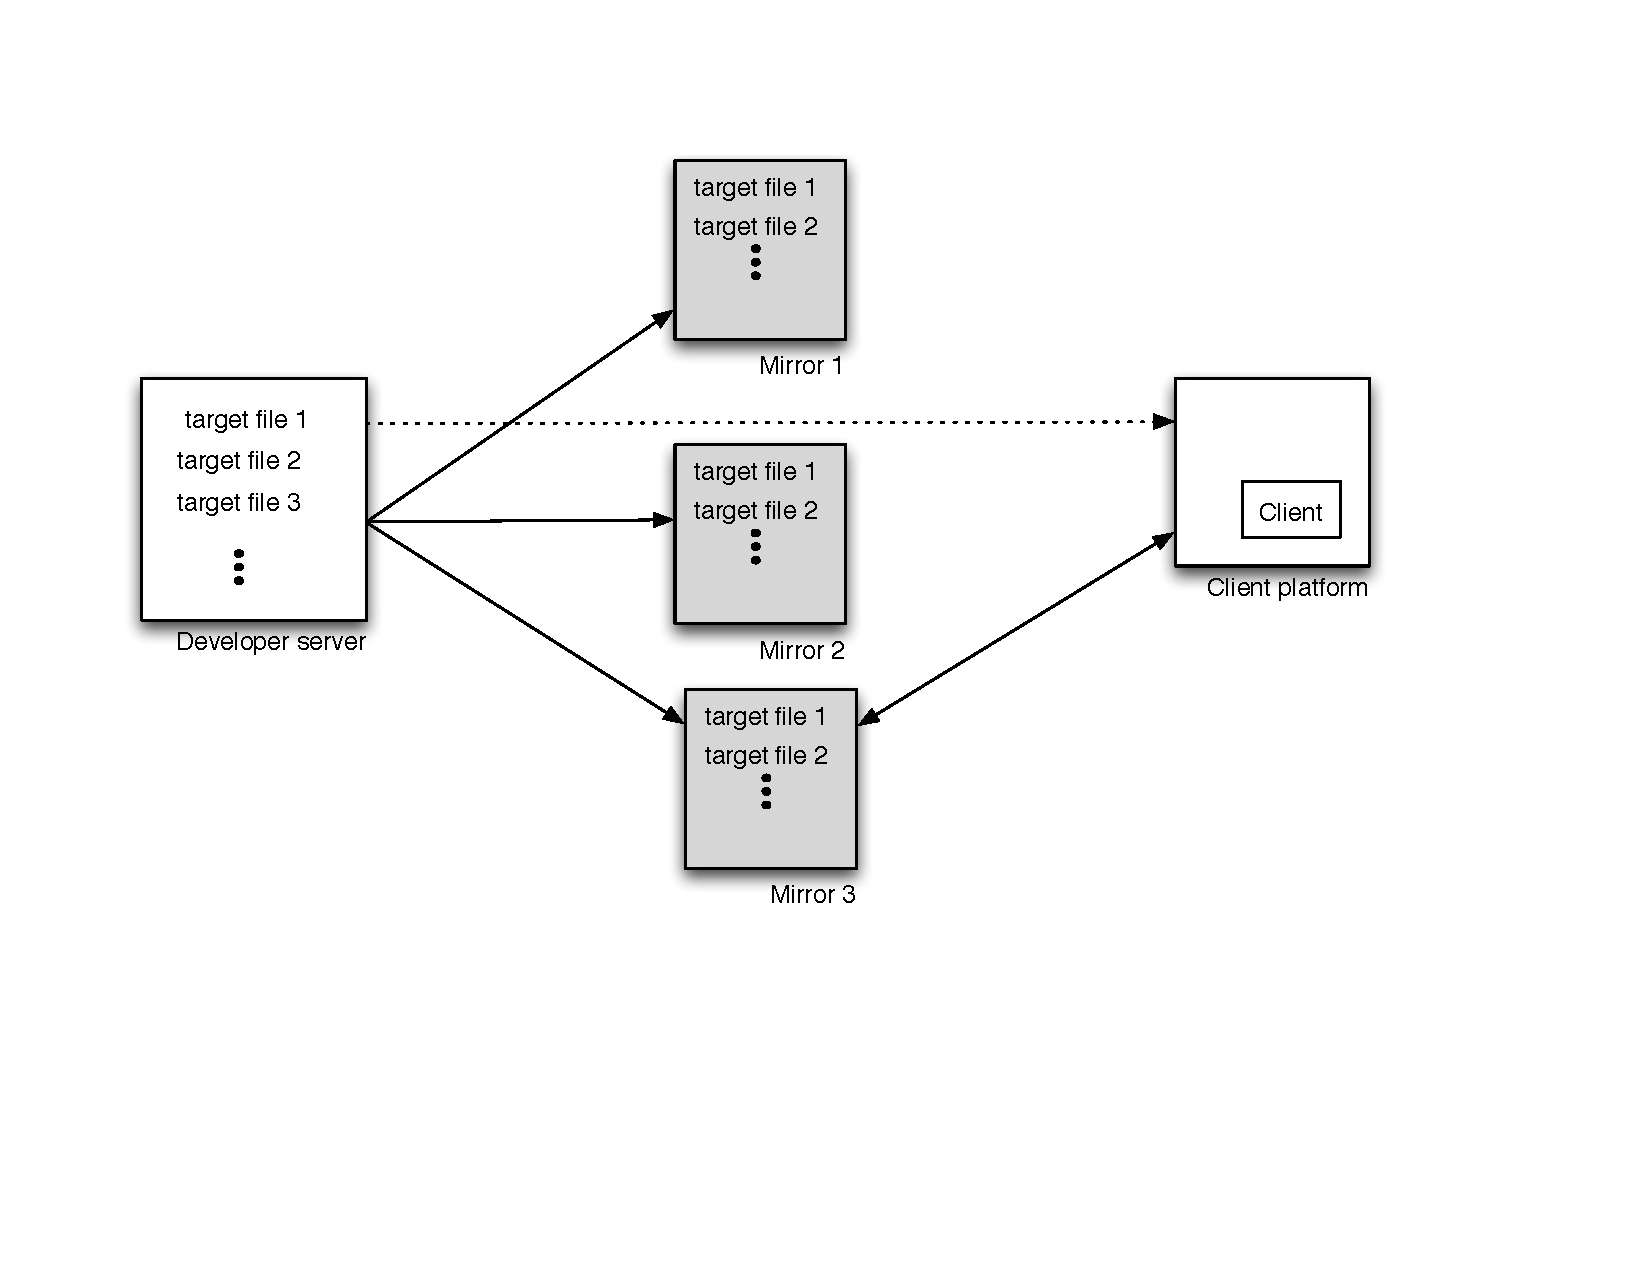
\includegraphics[width=0.7\textwidth]{Figures/update_platform.pdf}
 \captionsetup{font=footnotesize,justification=justified,singlelinecheck=false}
\caption{Modern software update platforms. The client obtain metadata from the trusted server for information about updates. The client then attempts to obtain the updates from one of the mirrors.}
\label{update_platform}
\end{figure*}
\indent The maintenance and security of modern applications depend on frequent system updates and patches.
% today more than ever.  With the increase in tools to prevent malware from infecting systems and the proliferation of devices requiring flexible underlying software, the software update process remains an important avenue available to attackers\cite{bellis01}.  
Since the updating process involves both communicating to  external entities and possibly running the update tools at an increased privilege level, it present a viable attack surface to harm not only the updating application, but the entire platform in general. In addition, since updates are the means by which software vulnerabilities in software systems are corrected, the lack of timely updates may enable vulnerabilities to be fully exploited even when the developers believed they have fixed the problem.

Figure \ref{update_platform} shows the general framework of current update systems. A cryptographic signatures of files to update (target files) is used to verify that their contents are accurate. The software developer
uses one ore multiple servers to store the most up to date target files. The files are then distributed to third party mirrors for faster deployment. The client \footnote{Throughout the rest of the paper, we refer to the application to be updated as client.} obtains the updates from the mirrors.  Work on the client side can be handled by package and library management systems, which works as an independent process and performs updates for different, unrelated clients, or through a self-updating process built in the client. 

Software update systems typically use a cryptographic signature of the files being updated target files to verify that the contents of the file are accurate. Though the targets are sent from mirrors using secure transmission protocols, this approach still leaves the client susceptible to various forms of attacks from the mirror\cite{tuf02}:
\begin{itemize}
\item{\emph{Rollback attacks}, where the client receives an update that is an older version of the target file.}
\item{\emph{Freeze attacks},  where the client receives notification of an update that has not actually occurred.}
\item{\emph{Mix \& match attacks},  where the client receives a valid partial update of due to a combination of metadata describing the target file that should never have existed.}
\item{\emph{Endless data attacks},  where the client receives an infinite stream of data when attempting an update.}
\item{\emph{Slow retrieval attacks},  where the client receives a valid update so slowly during an automated update that the vulnerability in the target remains indefinitely.}
\item{\emph{Extraneous dependency attacks},  where the client receives a valid update that incorrectly causes additional extraneous software to be downloaded due to invalid target requirements.}
\end{itemize}
As shown by Cappos et al.\ \cite{capp01}, the integrity and identity of software distribution mirrors for many popular software packages and operating systems is not verifiable in many cases.  Therefore, a reliable software update package must be able to function with the assumption that any mirror could be partially or fully responsible for an attack.

TUF  provides security against the attacks enumerated above by providing a multiple-signature trust model, an effective test for update recency and a separation of security responsibilities into distinct roles.   For \emph{�}xample, including timestamp information in update metadata files allows the client to verify that an update is more recent than the one that is currently active.  TUF allows for this metadata information to be compared to that in possession of the mirror site that it is interacting with to verify that the mirror is legitimate.  TUF has been designed so that it is relatively easy to introduce into the installation process of new software packages.  However, in order to use it in existing packages, modifications to the update configuration files or source code may be required.  This may not be possible in many situations, or if it is, pose enough of an obstacle to deter implementation in environments where security is not a priority.  TUF-Legacy provides an approach to overcome these obstacles by implementing a man-in-the-middle system to introduce the TUF security features without changes to existing update software.


\section{Background}
This section will briefly describe the existing TUF protocols and how they are implemented in a software update where TUF has been installed.
\section{Threat Model}
The threat model for TUF-Legacy is basically the same as that described by Cappos et al.\ \ref{tuf02} for the basic TUF system.  The model assumes that attackers can compromise at least one or more of a software system's trusted keys simultaneously or over a period of time, and that they can act as a transparent man-in-the-middle for client update requests.  An attack is considered successful if a client can be convinced to install something other than the most recent update available, or if the client is led to believe that the most recent update has been installed when in fact nothing has changed.  A key compromise is deemed to occur whenever an attacker can present to the client an arbitrary set of files with a matching key for those files since for all intensive purposes the use of the key on those files provides no evidence of the attack.

\section{Architecture}
\begin{figure*}[h!]
\centering
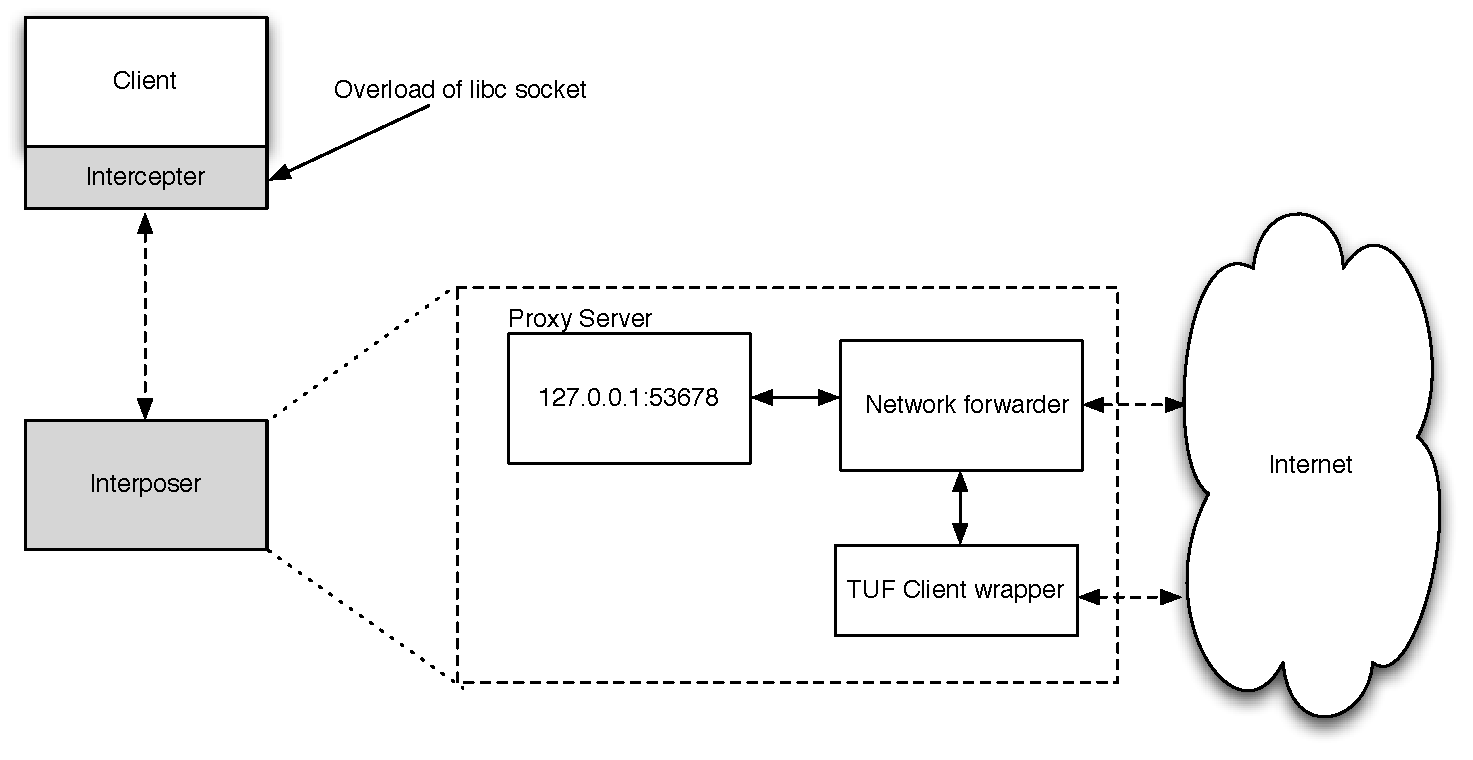
\includegraphics[width=0.8\textwidth]{Figures/Architecture.pdf}
 \captionsetup{font=footnotesize,justification=justified,singlelinecheck=false}
\caption{Architecture of proposed module. The dotted arrows represent network communications.} 
\label{tuf_legacy}
\end{figure*}

The primary idea behind the proposed module is to interpose itself between network communications of the client and the external world. Since network accesses related to software updates have two groups of contact (servers  and mirrors), the module can efficiently distinguish calls related to software updates (\emph{update calls}) and those that are not (\emph{misc calls}). Misc calls are forwarded to their destination and their  returned values are sent back to the client. Upon detecting an update call, the module calls a TUF wrapper to perform the security checks and to update the file requested. Figure \ref{tuf_legacy} details the different components of the module and their interactions.

\textbf{Intercepter.}  The interposer first intercepts network calls of the client. This is done by modifying kernel calls related to network communications (the socket library in libc) and loading the modified library (using \emph{LD\_PRELOAD} \cite{ld_preload}) to run alongside the client. The intercepter collects information about the network calls (i.e. function name and parameters) and sends the information to the proxy server.

\textbf{Proxy server.} The localhost  proxy server receives network calls between the client and the external world. Upon receiving requests from the intercepter loaded with the client client, the proxy server unpacks the parameters and calls the Network forwarder. %The local proxy server also returns network responses to the client. 

\textbf{Network forwarder.} The network forwarder takes the network call parameters (flags, socket type\ldots) and categorize them between update and misc calls (based on the ip address\footnote{The network forwarder has a dictionary  containing the IP address of the server and the supplying mirrors.}). The forwarder is also responsible to create, maintain and update the socket descriptor id for each network call. The descriptor is then returned to the proxy server, the intercepter and eventually back to the client. For misc calls, the forwarder works as tunnel between the client and the external world. For update calls, the forwarder uses  a TUF Client wrapper to perform the various security checks detailed in section 2.
\section{Implementation}
\section{Evaluation}
\section{Related Work}
\section{Conclusion}

\begin{thebibliography}{99}
\bibitem{ld_preload} http://www.kernel.org/doc/man-pages/online/pages/man8/ld-linux.so.8.html
\bibitem{bellis01}A. Bellisimo, John Burgess, and Kevin Fu,  ``Secure Software Updates: Disappointments and New Challenges",  In \emph{HotSec '06}, Vancouver, Canada, July 2006.
\bibitem{capp01} J. Cappos, J. Samuel, S. Baker, and J. Hartman, `` A Look In The Mirror:  Attacks on Package Managers",  In \emph{CCS '08}  Alexandria, Va., October 2008.
\bibitem{tuf02} J. Cappos and G. Condra, ``Secure Update Framework Repository Key Management and Trust Delegation", https://www.updateframework.com/browser/specs/tuf-spec.txt
%``Secure Update Framework Repository Key Management and Trust Delegation",  https://www.updateframework.com/browser/specs/tuf-spec.txt
\bibitem{liang01} Z. Liang, R. Sekar, W. Sun, and V.N. Venkatakrishnan, ``Expanding Malware Defense by Securing Software Installations",  In \emph{DIMVA'08}, Paris, France. July  2008.
\bibitem{tuf01} J. Samuel, N. Mathewson, J. Cappos, and R. Dingledine, ``Survivable Key Compromise in Software Update Systems",  In \emph{CCS' 10},  Chicago, IL, October 2010.

\end{thebibliography}

\end{document}
This is never printed